\documentclass{article}
\usepackage[utf8]{inputenc}
\usepackage[russian]{babel}
\usepackage{marginnote}
\usepackage{graphicx}
\usepackage{float}
\usepackage{makecell}
\usepackage{marginnote}
\usepackage{adjustbox}
\usepackage[table]{xcolor}
\usepackage{hyperref}

\hypersetup{
    colorlinks=true,
    linkcolor=blue,
    filecolor=magenta,      
    urlcolor=cyan,
}

\title{Базы данных. Лекция 13.}
\author{@mikhirurg }
\date{May 2020}

\begin{document}

\maketitle

\section{Базы знаний и онтологии.}

\subsection{База знаний}
Это совокупность единиц знаний, которые представляют собой формализованное с помощью некоторого метода представления знаний отражения объектов в проблемной области и их взаимосвязей, действий над объектами и, возможно, неопределённостей, с которыми эти действия осуществяются. 
\newline Знания в голове человека ощутимо всязаны с неопределённостью. 
\newline
\newline Базы знаний делятся на:
\begin{itemize}
    \item Замкнутые
    \item Открытые
\end{itemize}

\subsubsection{Логические модели}
\begin{itemize}
    \item Формальная система, задаваемая кортежем: \textit{M = <T, P, A, B>}
    \item \textit{T} - счётное множество базовых элементов (алфавит).
    \item \textit{P} - множество синтаксических правил (формул).
    \item \textit{A} - множество аксиом.
    \item \textit{B} - конечное множество правил вывода.
\end{itemize}
Пример: язык \textit{Prolog}
\begin{figure}[H]
    \centering
    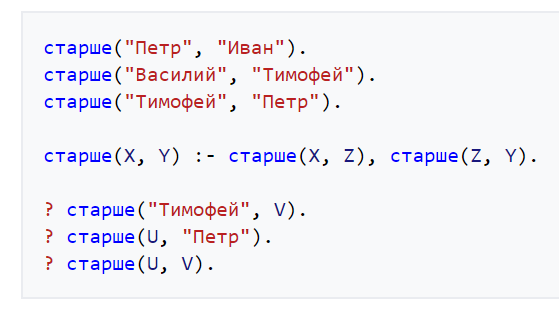
\includegraphics[width = .7\linewidth]{img0}
    \caption{Пример решения логической задачи на Prolog.}
\end{figure}

\subsubsection{Сетевые модели}
Формально может быть задана кортежем \textit{H = $<I, C_1, C_2, C_3, ..., C_n, G>$}
\begin{itemize}
    \item \textit{I} ~-- множество информационных единиц.
    \item \textit{$C_1, C_2, C_3, ..., C_n$} ~-- множество типов связей.
    \item \textit{G} ~-- отображение, задающее связи между единицами.
\end{itemize}
Типы сетей: 
\begin{itemize}
    \item Классифицирующие (используют связь ISA/AKO, APO)
    \item Функциональные (вычислительные)
    \item Сценарные (предпосылка - результат)
\end{itemize}

\subsection{Онтологии}
\begin{itemize}
    \item Форма представления семантической сети.
    \item Часто используется для терминологического базиса предметной области.
    \item Состав онтологии:
    \begin{itemize}
        \item Экземпляр
        \item Понятие
        \item Атрибут
        \item Отношение
    \end{itemize}
\end{itemize}

\subsubsection{Фреймовые модели}
\textbf{Фрейм} ~-- структура для описания стериотипной ситуации, состоящая из характеристик этой ситуации (слотов) и их значений
\newline
Значением слота может быть константа или процедура вычисления значения.
\newline
Виды процедур:
\begin{itemize}
    \item Если добавлено, то...
    \item Если удалено, то...
    \item Если нужно, то...
\end{itemize}
\textbf{Фасет} ~-- слот, принимающий множество значений.
\subsubsection{Продукционные модели}
\textbf{Если} \color{blue}<условие>\color{black} \textbf{То} \color{blue}<Заключение>\color{black} \textbf{CF} \textit{(Фактор определённости)} \color{blue}<значение>\color{black}
\newline
Формально может быть описана в виде кортежа \textit{$<I, Q, A\Rightarrow B, N>$}, где:
\begin{itemize}
    \item \textit{I} ~-- имя продукции
    \item \textit{Q} ~-- область применения продукции
    \item \textit{P} ~-- условие ядра продукции
    \item \textit{$A\Rightarrow B$} ~-- ядро продукции
    \item \textit{N} ~-- постусловие применения продукции
\end{itemize}
\end{document}